\documentclass{beamer}
\setbeamertemplate{navigation symbols}{}
\usepackage{beamerthemeshadow}
\usepackage{amsmath}
\usepackage{chronology}
\begin{document}

\title[Dashboard for MAB Algorithms]{Dashboard for Multi Armed Bandit (MAB) Algorithms}
\author[Surbhi Gupta, Kishan Patel]{Surbhi Gupta, Kishan Patel}
\date{November 13, 2013}

\begin{frame}
\titlepage
\begin{center}
Supervisor: Aditya Mahajan, Design Project 1
\end{center}
\end{frame}

\begin{frame}
\tableofcontents
\end{frame}

\section{Overview}

\subsection{Objective and Purpose}
\begin{frame}{Objective and Purpose}
\textbf{Objective}
\newline To build a \textbf{dashboard} in order to represent the results of executing a generic class of \textbf{Multi Armed Bandit} (MAB) algorithms used for \textbf{Website Optimization} (WO) 
\newline
\\\textbf{Purpose}
\\Ease of identification of best performing (most efficient) MAB algorithm for WO as well as
\begin{itemize}
  \item In-depth visual understanding
  \item Engaging interactive design
\end{itemize}
\end{frame}

\subsection{Terminology}
\begin{frame}{Terminology}
Some terms to familiarize with 
\begin{itemize}
  \item \textbf{Agent}: Decision maker
  \item \textbf{Arm}: Action 
  \item \textbf{Gain}: Measure of success or reward
\end{itemize}
\end{frame}

\subsection{MAB Problem and Algorithm}
\begin{frame}{MAB Problem}
\textbf{Problem}
\newline An \textbf{agent} chooses 1 \textbf{arm}, and receives a \textbf{gain} from it.
\newline How can the agent \textbf{maximize} his gain?
\newline
\newline \textbf{Algorithm}
\newline Look for the most optimal arm by
\begin{itemize}
  \item Exploiting the highest performing arms
  \item Exploring other arms to see if they perform even better
\end{itemize}
\end{frame}

\subsection{Website Optimization}
\begin{frame}{Website Optimization}
WO as a bandit problem
\newline
\newline What do each of these represent?
\begin{itemize}
  \item Agent: User
  \item Arm: Website version with unique styling
	\begin{itemize}
		\item Color scheme
		\item Layouts 
		\item Size of buttons
	\end{itemize}
  \item Gain: \textbf{Effectiveness} of a particular website version
	\begin{itemize}
		\item Effectiveness can be defined as a metric of success 
		\item Definition varies across domains
		\item Eg. 1 Number of purchases of a particular item on Amazon.com
		\item Eg. 2 Number of donors on a fundraising website
	\end{itemize}
\end{itemize}
\end{frame}

\section{Progress till date}

\subsection{Project Execution Overview}
\begin{frame}{Project Execution Overview}
\begin{enumerate}
	\item Introduction to MAB
	\item Model WO as a MAB problem
	\item Identify the purpose of a creating a dashboard 
	\begin{itemize}
		\item Research to choose a suitable charting library
		\item Create graphs using the chosen library
		\item Discuss feedback with supervisor
	\end{itemize}
	\item Next steps
	\begin{itemize}
		\item Prioritize requirements and visit backlog
		\item Create a tentative timeline for next semester
	\end{itemize}
\end{enumerate}
\end{frame}

\subsection{Charting Library Research}
\begin{frame}{Charting Library Research}
	\begin{itemize}
		\item Options explored: Radian, Cubism.js, NVD3.js, Rickshaw
		\item Narrowed choices to: Radian, Rickshaw
	\end{itemize}
\end{frame}

\begin{frame}{Radian}
\begin{tabular}{| p{2.5cm} | p{8cm} |}
    \hline
     \textbf{Parameter} & \textbf{Radian} \\ \hline
  \textbf{Reliability} \newline & In development phase\newline Released in 2013 (very new) \\ \hline
  \textbf{Resource \newline Availability} &  Well organized tutorial documentation
		\newline External resources for Angular.js directives 
		\newline Untidy and non-intuitive Github repository \\ \hline
  \textbf{Learning Curve} &  Knowledge of HTML
		\newline Custom HTML elements can represent functional and data plots
		\newline Angular.js knowledge for interactive plots \\ \hline
\textbf{Features and Extensibility}& Limited basic features (covered by Rickshaw) \\ \hline
\end{tabular}
\end{frame}

\begin{frame}{Rickshaw}
\begin{tabular}{| p{2.5cm} | p{8cm} |}
    \hline
     \textbf{Parameter} & \textbf{Rickshaw} \\ \hline
\textbf{Reliability}\newline & Established framework\newline Released in 2011 \\ \hline
\textbf{Resource \newline Availability} &  Limited and concise tutorial documentation
		\newline Comprehensive '/examples' section in Github repository\\ \hline
\textbf{Learning Curve}  &  Knowledge of JavaScript for functional, data and interactive plots \\ \hline
\textbf{Features and Extensibility} & Feature rich
		\newline Vast range of extensions to build on and extend existing functionality\\ \hline
\end{tabular}
\end{frame}

\begin{frame}{Charting Library Research: Result}
\begin{itemize}
	\item Final choice: Rickshaw
	\item Increased reliability- more established framework
	\item Enhanced resource availability- comprehensive Github repository
	\item Neutral learning curve
		\begin{itemize}
			\item Common skill between group members- JavaScript
			\item Limited time to learn a new framework (Angular.js)
		\end{itemize}
	\item Rich feature set
		\begin{itemize}
			\item Wide range of extensions to customize (suitable for our project)
			\item Eg. Time fixture feature for incorporating time series graphs
		\end{itemize}
\end{itemize}
\end{frame}

\subsection{Implemented Graphs and Features}
\begin{frame}{File Upload}
 	\begin{itemize}
   		\item The results of the simulation is saved in a file
		\item Most basic file contains information about each clock tick (arm selected and result achieved)
		\item Multiple formats supported: CSV, JSON, Tabular
		\item Once file is loaded, charts are generated
		\item The end objective is to support live data in addition to file upload
	\end{itemize}
\end{frame}

\begin{frame}{File Upload - Bar Chart}
\begin{itemize}
\item The bar chart simply represents the data at each clock tick - A 1 or 0. 
\item In this example, for the first three clock ticks, there was no gain for any arm. For the next three clock ticks, arm 1 resulted in a reward and for the last two clock ticks, arm 2 resulted in a reward.
\end{itemize}
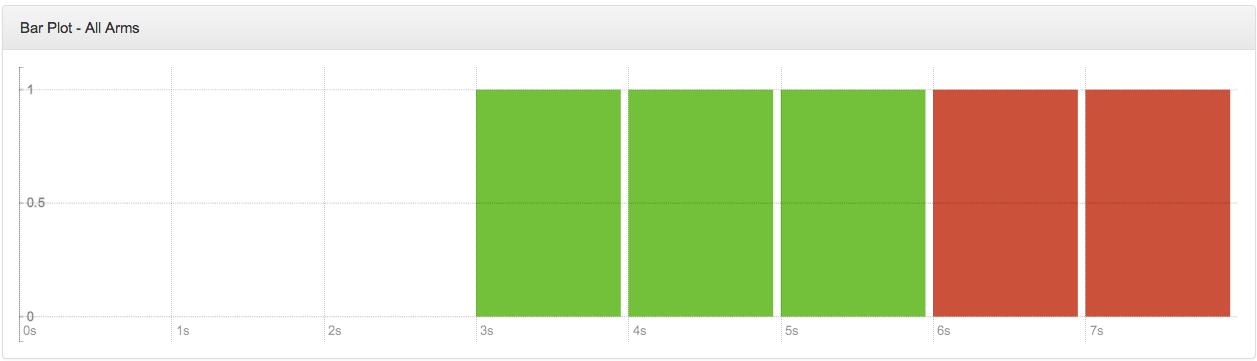
\includegraphics[scale=0.25]{barchart.png}
\end{frame}

\begin{frame}{File Upload - Line Chart}
\begin{itemize}
\item The line chart represents the average reward received over time
\item Each point on the line represents the number of times the arm was played divided by the total time elapsed
\end{itemize}
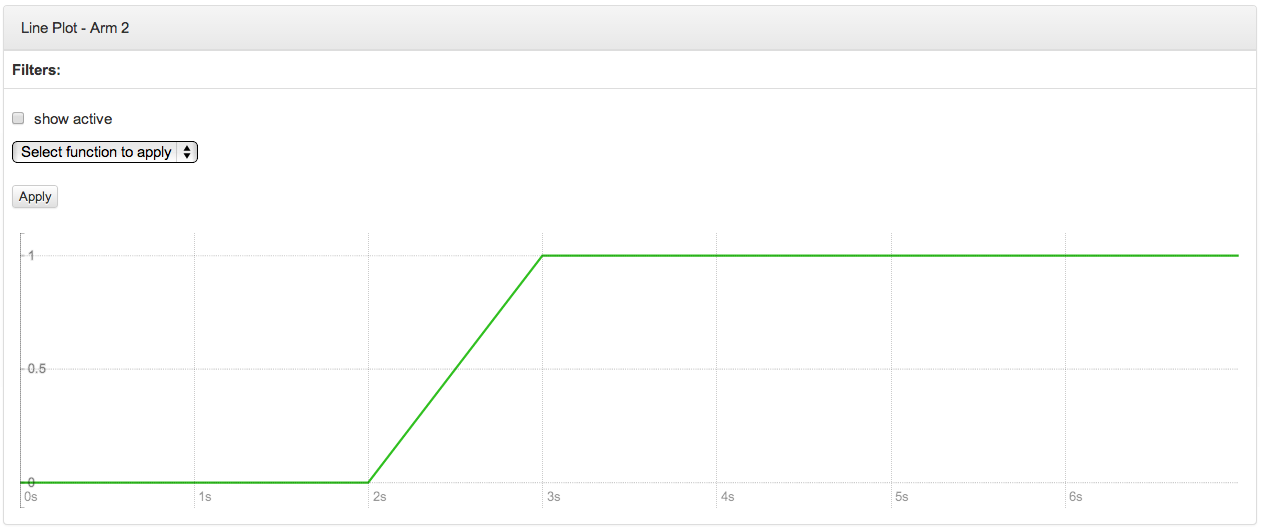
\includegraphics[scale=0.25]{linechart.png}
\end{frame}

\begin{frame}{Arm Details}
\begin{itemize}
\item Ability to differentiate between time arm was active/unactive
\end{itemize}
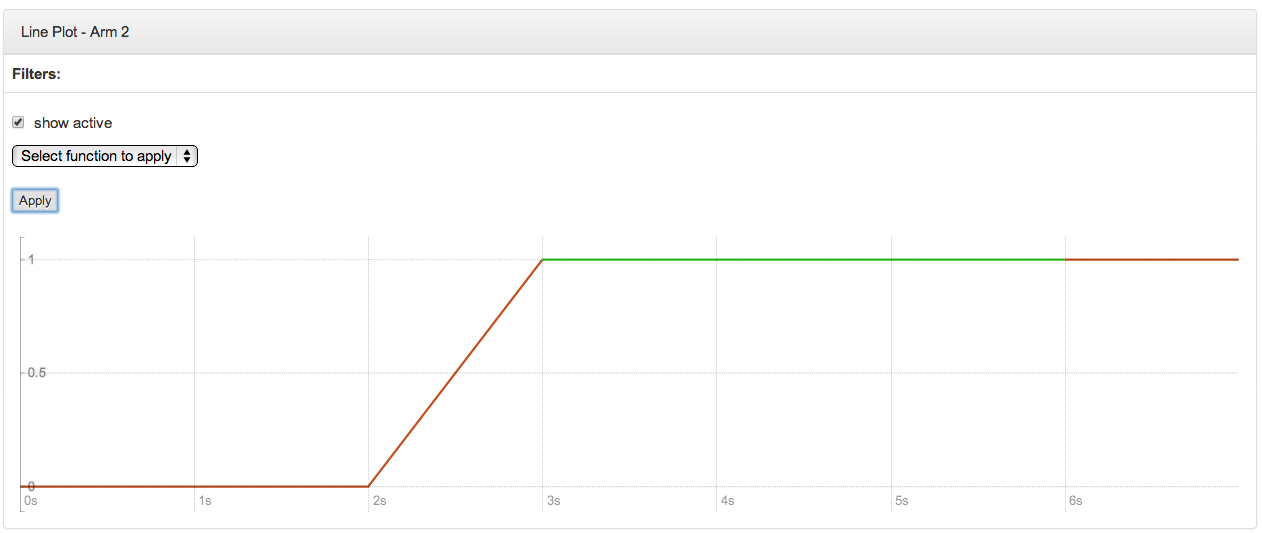
\includegraphics[scale=0.25]{linechartactive.png}
\end{frame}

\begin{frame}{Viewing Results by Time}
\begin{itemize}
\item For website optimization, traffic varies by time of day
\item In order to normalize time zones, bar chart displays results by hour
\end{itemize}
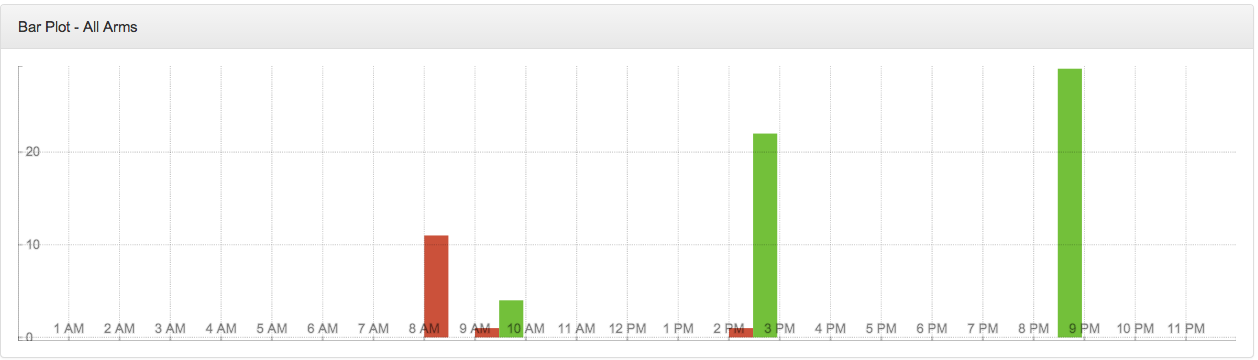
\includegraphics[scale=0.25]{barcharttime.png}
\end{frame}

\begin{frame}{Applying a Function}
\begin{itemize}
\item Function is applied to the static data to generate a simulated line
\item Some functions include: UCB, Epsilon Greedy
\end{itemize}
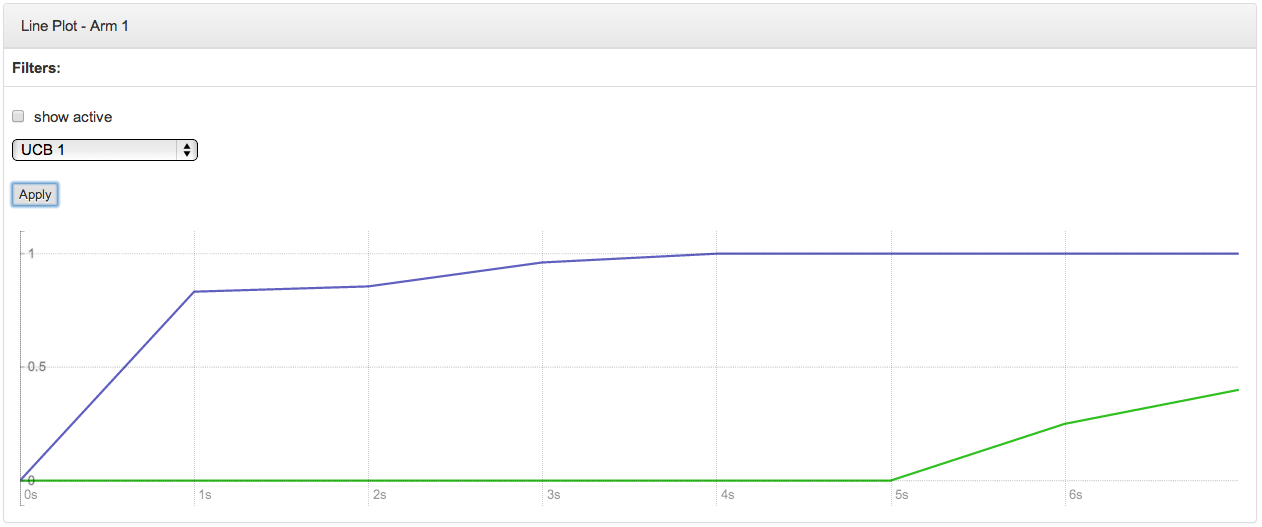
\includegraphics[scale=0.25]{linechartfunction.png}
\end{frame}

\section{Future Plans}

\subsection{Features to be added}
\begin{frame}{Support for Live Data and Enhanced Interactivity}
\begin{itemize}
\item Next major goal is to add support for live data
\item The application would listen to events sent by some client and produce graphs in realtime
\item The idea is to support multiple clients each having their own graphs
\item Increase in interactivity includes: hover effects, adding a slider to accomodate for large data and adding more filtering options
\item Define a common interface to communicate with the Web Application
\end{itemize}
\end{frame}

\subsection{Timeline}
\begin{frame}{Timeline}
\textbf{DP1, Fall 2013}:
\begin{itemize}
\item Make sure file upload is robust - all features discussed during meeting are fully implemented and functional
\item UI enhancements - filter and hover effects
\item Commence live stream implementation planning
\end{itemize}
\textbf{DP2, Winter 2014}:
\begin{itemize}
\item Complete live stream implementation
\item Add additional features (as needed)
\end{itemize}
\end{frame}


\section{Organization}

\subsection{Communication}
\begin{frame}{Communication}
\begin{itemize}
\item Primary forms of communication: emails and text messages
\item Source code repository: Github. Houses the backlog which consists of list of existing tasks and new tasks are added as progress is made
\item Dropbox : documents (meeting notes, resources and submissions)
\item Software process models like Waterfall or Agile are not used
\end{itemize}
\end{frame}

\subsection{Issue Tracker}
\begin{frame}{Issue Tracker}
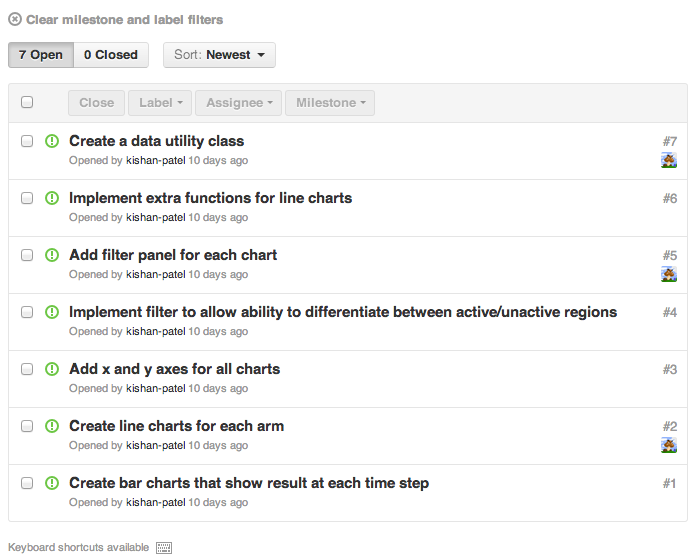
\includegraphics[scale=0.25]{gitissues.png}
\end{frame}

\subsection{Challenges}
\begin{frame}{Challenges}
\begin{itemize}
\item Higher learning curve in terms of development and testing with limited time resources
\item Development:  Adding support for multiple clients and live streaming
\item Testing: First time testing a web application 
	\begin{itemize}
		\item Familiarize with existing web testing tools
		\item Building variety of web test cases
		\item Detailed procedure covering functionality, usability, interface and compatibility, performance testing
	\end{itemize}
\item Successful implementation of dashboard along with robust testing
\end{itemize}
\end{frame}
\end{document}